\documentclass{standalone}
\usepackage{tikz}
\usetikzlibrary{patterns, positioning}
\usepackage[sfdefault]{ClearSans} %% option 'sfdefault' activates Clear Sans as the default text font
\usepackage[T1]{fontenc}

\begin{document}
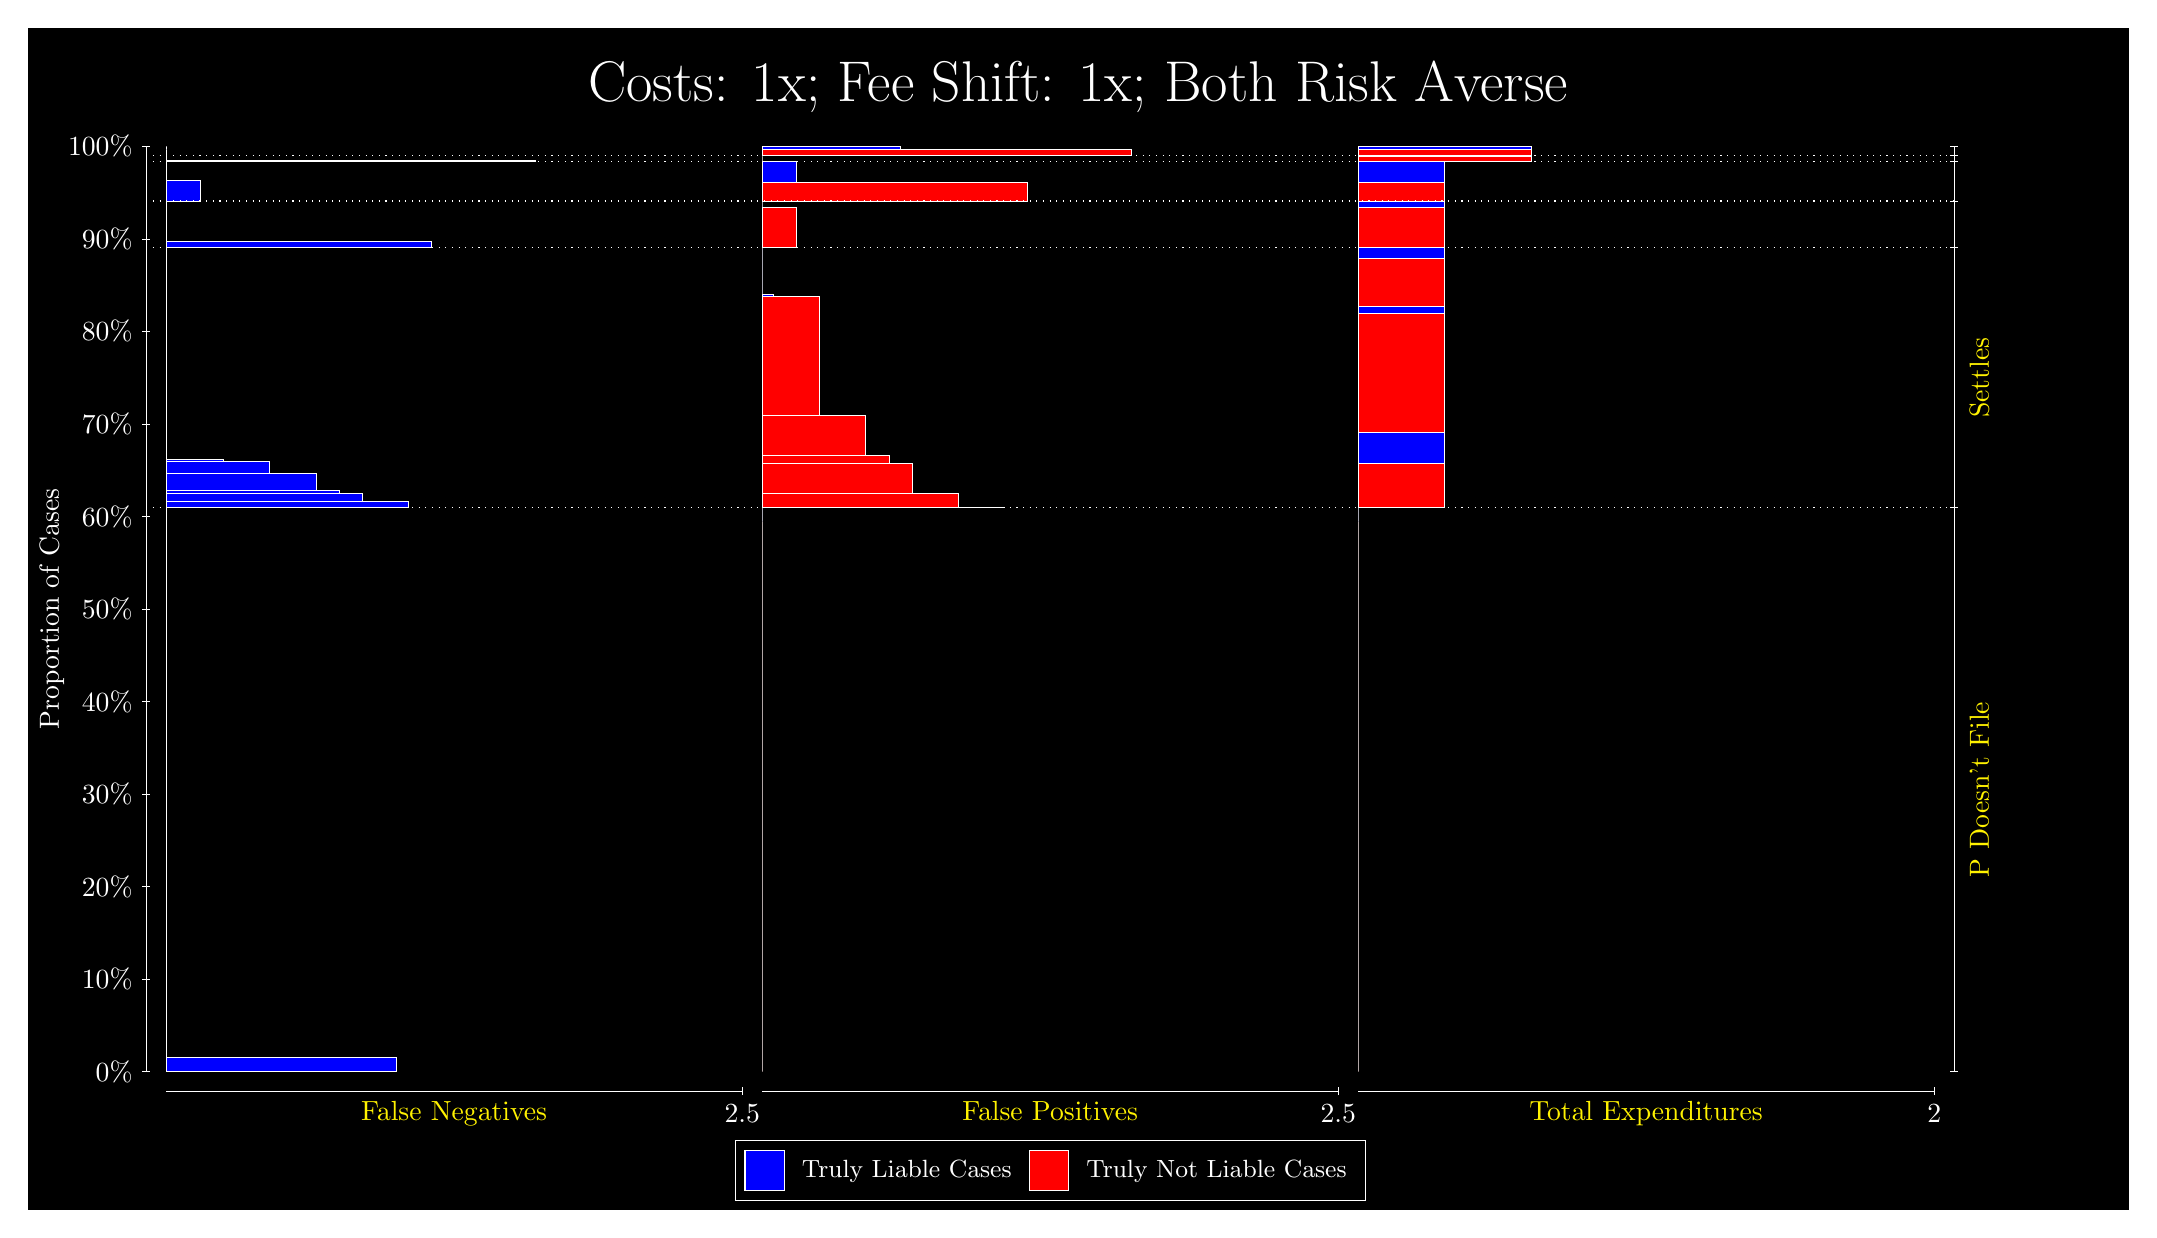
\begin{tikzpicture}
\draw[fill=black] (0,0) rectangle (26.667,15);
\draw[text=white] (0,13.5) rectangle (26.667,15) node[midway] {\huge Costs: 1x; Fee Shift: 1x; Both Risk Averse};
\draw[white, very thin] (1.5,1.75) -- (1.5,13.5);
\node[rotate=90, text=white, anchor=center] at (0.3, 7.625) {Proportion of Cases};
\draw[white, very thin] (1.45,1.75) -- (1.55,1.75);
\node[text=white, anchor=east] at (1.45, 1.75) {0\%};
\draw[white, very thin] (1.45,2.925) -- (1.55,2.925);
\node[text=white, anchor=east] at (1.45, 2.925) {10\%};
\draw[white, very thin] (1.45,4.1) -- (1.55,4.1);
\node[text=white, anchor=east] at (1.45, 4.1) {20\%};
\draw[white, very thin] (1.45,5.275) -- (1.55,5.275);
\node[text=white, anchor=east] at (1.45, 5.275) {30\%};
\draw[white, very thin] (1.45,6.45) -- (1.55,6.45);
\node[text=white, anchor=east] at (1.45, 6.45) {40\%};
\draw[white, very thin] (1.45,7.625) -- (1.55,7.625);
\node[text=white, anchor=east] at (1.45, 7.625) {50\%};
\draw[white, very thin] (1.45,8.8) -- (1.55,8.8);
\node[text=white, anchor=east] at (1.45, 8.8) {60\%};
\draw[white, very thin] (1.45,9.975) -- (1.55,9.975);
\node[text=white, anchor=east] at (1.45, 9.975) {70\%};
\draw[white, very thin] (1.45,11.15) -- (1.55,11.15);
\node[text=white, anchor=east] at (1.45, 11.15) {80\%};
\draw[white, very thin] (1.45,12.325) -- (1.55,12.325);
\node[text=white, anchor=east] at (1.45, 12.325) {90\%};
\draw[white, very thin] (1.45,13.5) -- (1.55,13.5);
\node[text=white, anchor=east] at (1.45, 13.5) {100\%};

\draw[white, very thin] (24.457,1.75) -- (24.457,13.5);
\draw[white, very thin] (24.407,1.75) -- (24.507,1.75);
\node[anchor=west] at (24.407, 1.75) {};
\draw[white, very thin] (24.407,8.9096) -- (24.507,8.9096);
\node[anchor=west] at (24.407, 8.9096) {};
\draw[white, very thin] (24.407,12.215) -- (24.507,12.215);
\node[anchor=west] at (24.407, 12.215) {};
\draw[white, very thin] (24.407,12.805) -- (24.507,12.805);
\node[anchor=west] at (24.407, 12.805) {};
\draw[white, very thin] (24.407,13.309) -- (24.507,13.309);
\node[anchor=west] at (24.407, 13.309) {};
\draw[white, very thin] (24.407,13.381) -- (24.507,13.381);
\node[anchor=west] at (24.407, 13.381) {};
\draw[white, very thin] (24.407,13.5) -- (24.507,13.5);
\node[anchor=west] at (24.407, 13.5) {};

\draw[white, very thin, fill=blue] (1.75,1.75) rectangle (4.6775,1.9249);
\draw[white, very thin, fill=red] (1.75,1.9249) rectangle (1.75,8.9096);
\draw[white, very thin, fill=blue] (1.75,8.9096) rectangle (4.8239,8.99);
\draw[white, very thin, fill=blue] (1.75,8.99) rectangle (4.2384,9.0972);
\draw[white, very thin, fill=blue] (1.75,9.0972) rectangle (3.9457,9.1295);
\draw[white, very thin, fill=blue] (1.75,9.1295) rectangle (3.6529,9.3449);
\draw[white, very thin, fill=blue] (1.75,9.3449) rectangle (3.0674,9.5056);
\draw[white, very thin, fill=blue] (1.75,9.5056) rectangle (2.4819,9.5239);
\draw[white, very thin, fill=red] (1.75,9.5239) rectangle (1.75,12.215);
\draw[white, very thin, fill=blue] (1.75,12.215) rectangle (5.1167,12.292);
\draw[white, very thin, fill=red] (1.75,12.292) rectangle (1.75,12.805);
\draw[white, very thin, fill=blue] (1.75,12.805) rectangle (2.1891,13.065);
\draw[white, very thin, fill=red] (1.75,13.065) rectangle (1.75,13.309);
\draw[white, very thin, fill=blue] (1.75,13.309) rectangle (6.4341,13.317);
\draw[white, very thin, fill=red] (1.75,13.317) rectangle (1.75,13.381);
\draw[white, very thin, fill=red] (1.75,13.381) rectangle (1.75,13.459);
\draw[white, very thin, fill=blue] (1.75,13.459) rectangle (1.75,13.5);
\draw[white, very thin, fill=red] (9.3189,1.75) rectangle (9.3189,8.7348);
\draw[white, very thin, fill=blue] (9.3189,8.7348) rectangle (9.3189,8.9096);
\draw[white, very thin, fill=red] (9.3189,8.9096) rectangle (12.393,8.9216);
\draw[white, very thin, fill=red] (9.3189,8.9216) rectangle (11.807,9.0929);
\draw[white, very thin, fill=red] (9.3189,9.0929) rectangle (11.222,9.4712);
\draw[white, very thin, fill=red] (9.3189,9.4712) rectangle (10.929,9.5734);
\draw[white, very thin, fill=red] (9.3189,9.5734) rectangle (10.636,10.081);
\draw[white, very thin, fill=red] (9.3189,10.081) rectangle (10.051,11.601);
\draw[white, very thin, fill=blue] (9.3189,11.601) rectangle (9.4652,11.619);
\draw[white, very thin, fill=blue] (9.3189,11.619) rectangle (9.3189,12.215);
\draw[white, very thin, fill=red] (9.3189,12.215) rectangle (9.758,12.729);
\draw[white, very thin, fill=blue] (9.3189,12.729) rectangle (9.3189,12.805);
\draw[white, very thin, fill=red] (9.3189,12.805) rectangle (12.686,13.049);
\draw[white, very thin, fill=blue] (9.3189,13.049) rectangle (9.758,13.309);
\draw[white, very thin, fill=red] (9.3189,13.309) rectangle (9.3189,13.372);
\draw[white, very thin, fill=blue] (9.3189,13.372) rectangle (9.3189,13.381);
\draw[white, very thin, fill=red] (9.3189,13.381) rectangle (14.003,13.459);
\draw[white, very thin, fill=blue] (9.3189,13.459) rectangle (11.075,13.5);
\draw[white, very thin, fill=red] (16.888,1.75) rectangle (16.888,8.7348);
\draw[white, very thin, fill=blue] (16.888,8.7348) rectangle (16.888,8.9096);
\draw[white, very thin, fill=red] (16.888,8.9096) rectangle (17.986,9.4712);
\draw[white, very thin, fill=blue] (16.888,9.4712) rectangle (17.986,9.8656);
\draw[white, very thin, fill=red] (16.888,9.8656) rectangle (17.986,11.385);
\draw[white, very thin, fill=blue] (16.888,11.385) rectangle (17.986,11.466);
\draw[white, very thin, fill=red] (16.888,11.466) rectangle (17.986,12.076);
\draw[white, very thin, fill=blue] (16.888,12.076) rectangle (17.986,12.215);
\draw[white, very thin, fill=red] (16.888,12.215) rectangle (17.986,12.729);
\draw[white, very thin, fill=blue] (16.888,12.729) rectangle (17.986,12.805);
\draw[white, very thin, fill=red] (16.888,12.805) rectangle (17.986,13.049);
\draw[white, very thin, fill=blue] (16.888,13.049) rectangle (17.986,13.309);
\draw[white, very thin, fill=red] (16.888,13.309) rectangle (19.083,13.372);
\draw[white, very thin, fill=blue] (16.888,13.372) rectangle (19.083,13.381);
\draw[white, very thin, fill=red] (16.888,13.381) rectangle (19.083,13.459);
\draw[white, very thin, fill=blue] (16.888,13.459) rectangle (19.083,13.5);
\draw[white, dotted] (1.5,8.9096) -- (24.457,8.9096);
\draw[white, dotted] (1.5,12.215) -- (24.457,12.215);
\draw[white, dotted] (1.5,12.805) -- (24.457,12.805);
\draw[white, dotted] (1.5,13.309) -- (24.457,13.309);
\draw[white, dotted] (1.5,13.381) -- (24.457,13.381);
\draw[white, very thin] (1.75,1.5) -- (9.0689,1.5);
\node[text=yellow, anchor=north] at (5.4094, 1.5) {False Negatives};
\draw[white, very thin] (9.0689,1.45) -- (9.0689,1.55);
\node[text=white, anchor=north] at (9.0689, 1.45) {2.5};

\draw[white, very thin] (9.3189,1.5) -- (16.638,1.5);
\node[text=yellow, anchor=north] at (12.978, 1.5) {False Positives};
\draw[white, very thin] (16.638,1.45) -- (16.638,1.55);
\node[text=white, anchor=north] at (16.638, 1.45) {2.5};

\draw[white, very thin] (16.888,1.5) -- (24.207,1.5);
\node[text=yellow, anchor=north] at (20.547, 1.5) {Total Expenditures};
\draw[white, very thin] (24.207,1.45) -- (24.207,1.55);
\node[text=white, anchor=north] at (24.207, 1.45) {2};

\node[text=yellow, centered, rotate=90] at (24.777, 5.3298) {P Doesn't File};
\node[text=yellow, centered, rotate=90] at (24.777, 10.562) {Settles};





\draw (12.978300999999998,1.5) node[draw=none] (baseCoordinate) {};
\begin{scope}[align=center]
        \matrix[scale=0.5, draw=white, below=0.5cm of baseCoordinate, nodes={draw}, column sep=0.1cm]{
            \node[rectangle, draw, minimum width=0.5cm, minimum height=0.5cm, fill=blue] {}; &
            \node[draw=none, font=\small, text=white] (B) {Truly Liable Cases}; &
            \node[rectangle, draw, minimum width=0.5cm, minimum height=0.5cm, fill=red] {}; &
            \node[draw=none, font=\small, text=white] (B) {Truly Not Liable Cases}; \\
            };
\end{scope}

\end{tikzpicture}
\end{document}